\scanpage{128}
$x$ maximal dans $\varphi_i^{-1}(\unsure{x_i})$

\diagram{\begin{tikzcd}[ampersand replacement=\&,column sep=small,row sep=small,execute at end picture={\draw[rounded corners] ([xshift=-8pt,yshift=8pt]\tikzcdmatrixname-1-2.north west) rectangle ([xshift=5pt,yshift=-8pt]\tikzcdmatrixname-2-4.south east);}]
\& (\text{Ép})' \arrow[r,Rightarrow] \arrow[dr,Rightarrow] \& (\text{Ép})+(\uline{\unsure{\text{unicité : fibre de }x_i}}) \& \\
\& \deleted{(\text{Ép})'''} \& (\text{Ép})''' \arrow[r,Rightarrow] \& \begin{gathered}\text{si }\deleted{\unsure{\forall x'_i}}X'_i,\ \exists\text{ un ouvert }\ne\varnothing\\ U_i\subset\bar x_i\text{ t.q. les }\varphi_{ij}^{-1}(U_i)\unsure{\times|\cap}X'_j=\varphi_j(X)\end{gathered}\quad ??? \\
(\text{Ép})'' \arrow[uur,Rightarrow,"\substack{\text{M.L.}\\\text{et }I=\mathbf N}"] \arrow[urr,Rightarrow,"4"'] \& \& \&
\end{tikzcd}}

\margin{$\deleted{\unsure{E}}\quad\text{p\textsuperscript{t} épais}\longleftarrow\substack{\text{\unsure{fermés} constructibles}\\\text{irréductibles}}$}

\[
U_j\cap X'_j\subset\bar x_j\qquad X'_i\longleftarrow X'_j
\]
\[
U_i\subset\bar x_i
\]
\margin{$x\in E\subset\bar x$}
\margin{$x\in U_0\cap Z_0$}
\margin{$\bar x$}

\[
x\in\deleted{\unsure{\bar x}}\bigcup_i U_i\cap Z_i
\]
\diagram{\begin{tikzcd}[ampersand replacement=\&,column sep=small,row sep=large]
\unsure{\mathcal X|\mathfrak X} \arrow[dr] \& \& \unsure{\mathcal X_i|\mathfrak X_i} \arrow[dl] \\
\& {} \&
\end{tikzcd}}

\[
x\in U_0\cap Z_0\subset\bar x
\]
\[
\deleted{\bar x\unsure{\in}\ \unsure{x_0}\in Z_0}\qquad
\bar x=\overline{U_0}\cap Z_0\subset Z_0
\]
$\unsure{U_0}$

$f_1\quad f_n$ \unsure{nuls en} $x$
\[
f_1\cdots f_n\in p\qquad g
\]
\[
\text{si }g\notin q\qquad q\supset p\Longleftrightarrow q\supset f_1\cdots f_n
\]
\figure{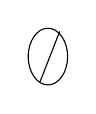
\begin{tikzpicture}\draw (0,0) ellipse (.25 and .36);\draw (-.1,-.32)--(.15,.32);\end{tikzpicture}}
\[
\mathcal O_{X,x}\qquad \unsure{\mathfrak m|m}_x\quad\deleted{\text{\unsure{idéal}}}
\]
$A_g$: un \unsure{idéal de définition}

\margin{\unsure{idéal de} \deleted{\unsure{type}} \unsure{un} \unsure{type fini} \unsure{d'où}}
\margin{127}
